\section{Storage Layer}


\begin{frame}
    \frametitle{ Components}
    \begin{figure}
        \centering
        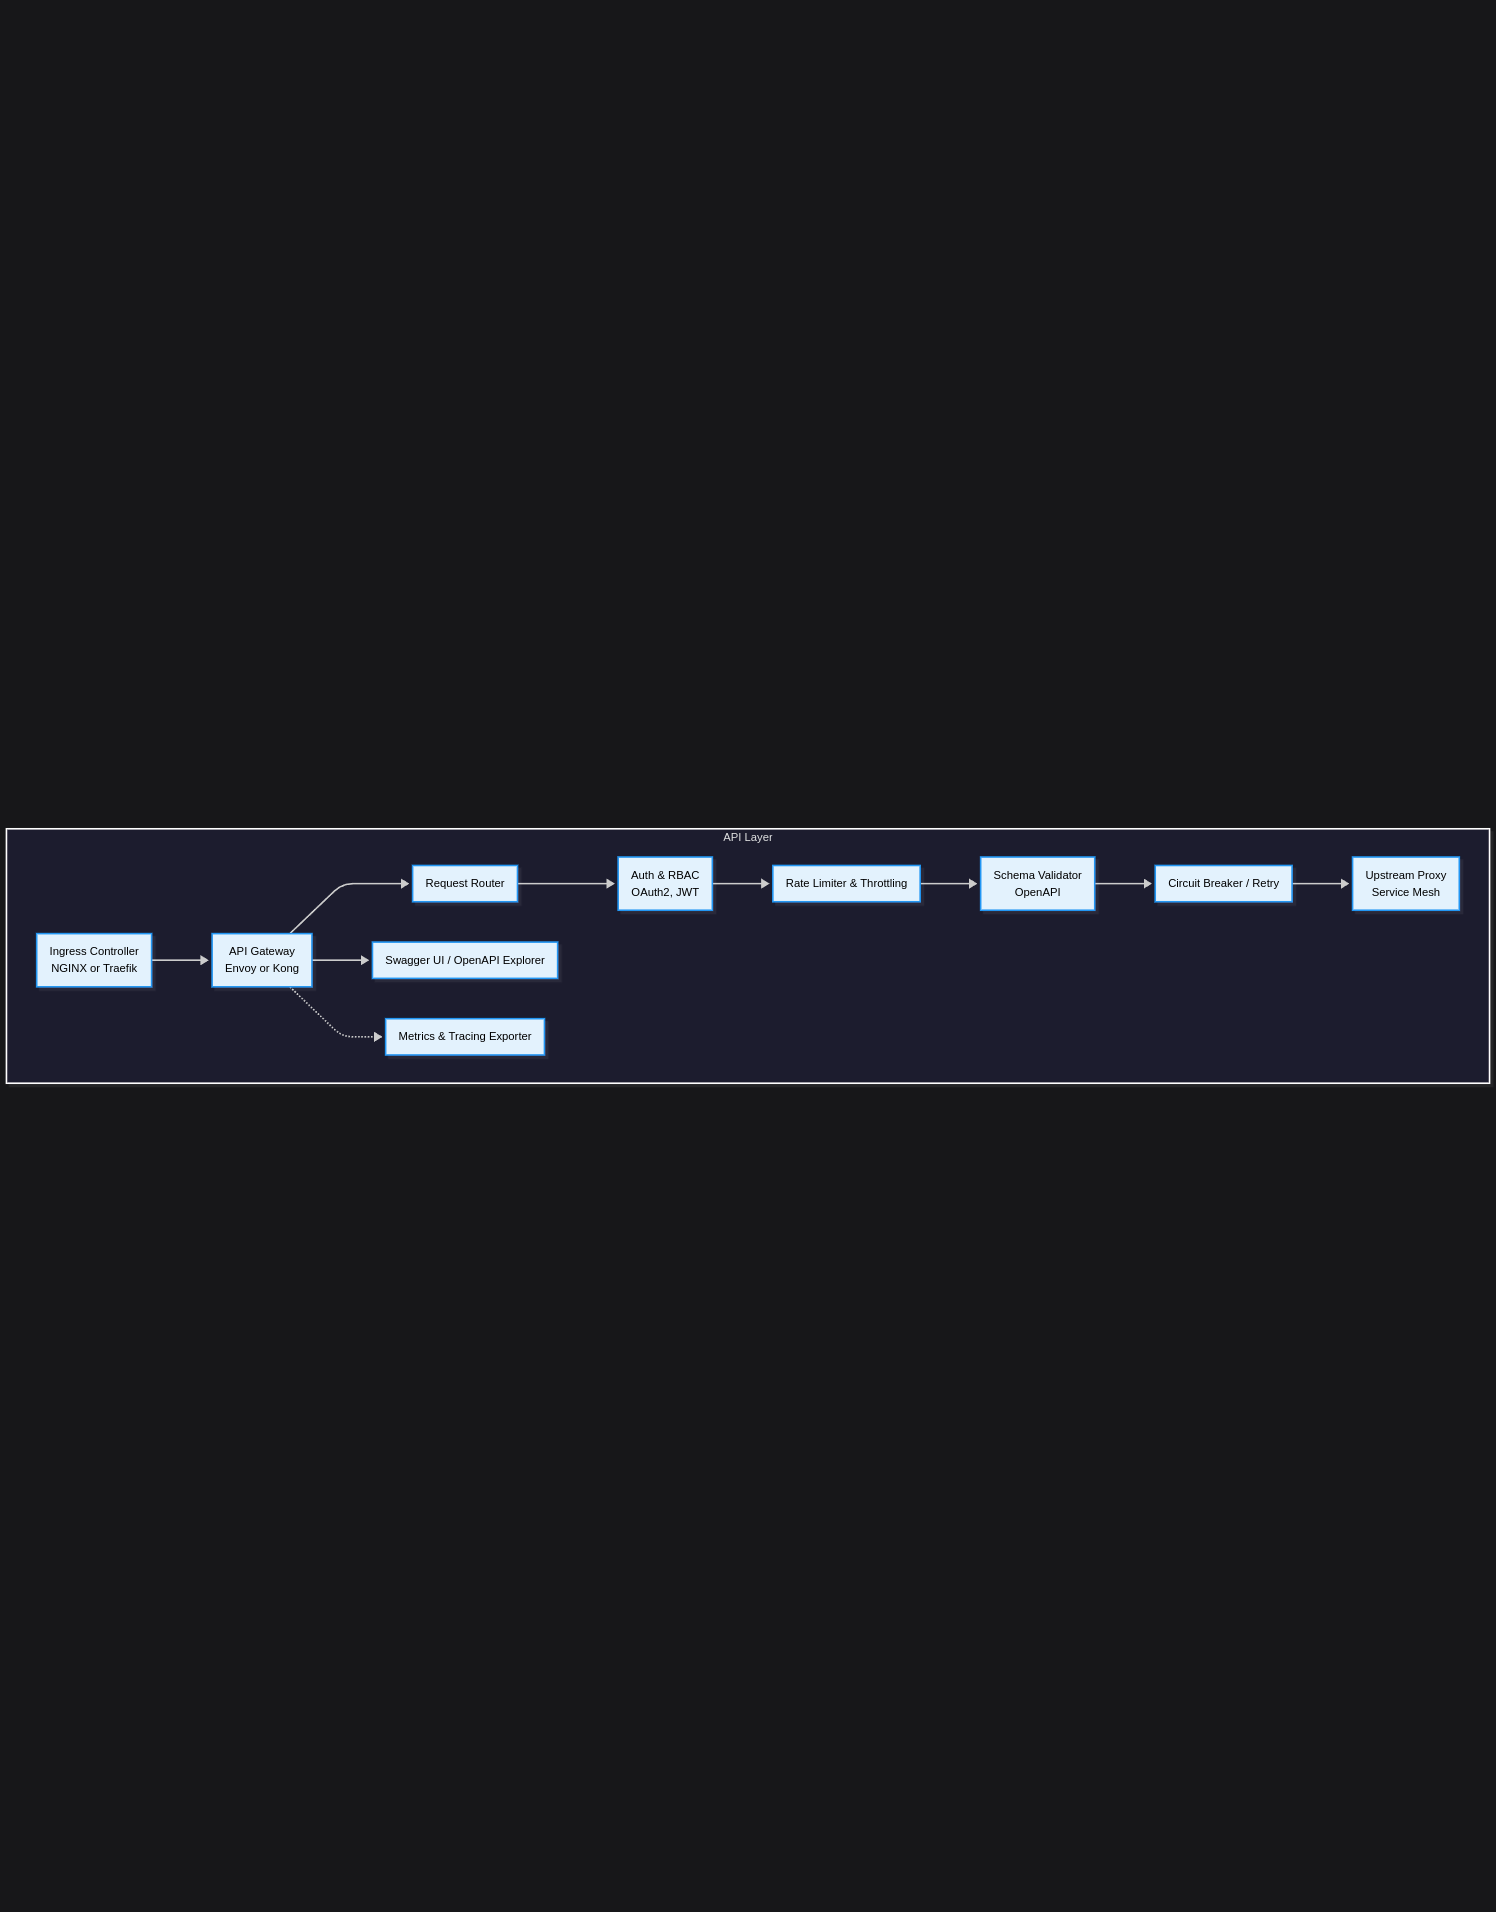
\includegraphics[width=0.5\textwidth]{store/layout.png} % Adjusted the scale of the image to 0.5
       
    \end{figure}
\end{frame}

% \begin{frame}
%     \frametitle{Flow}
%     \begin{figure}
%         \centering
%         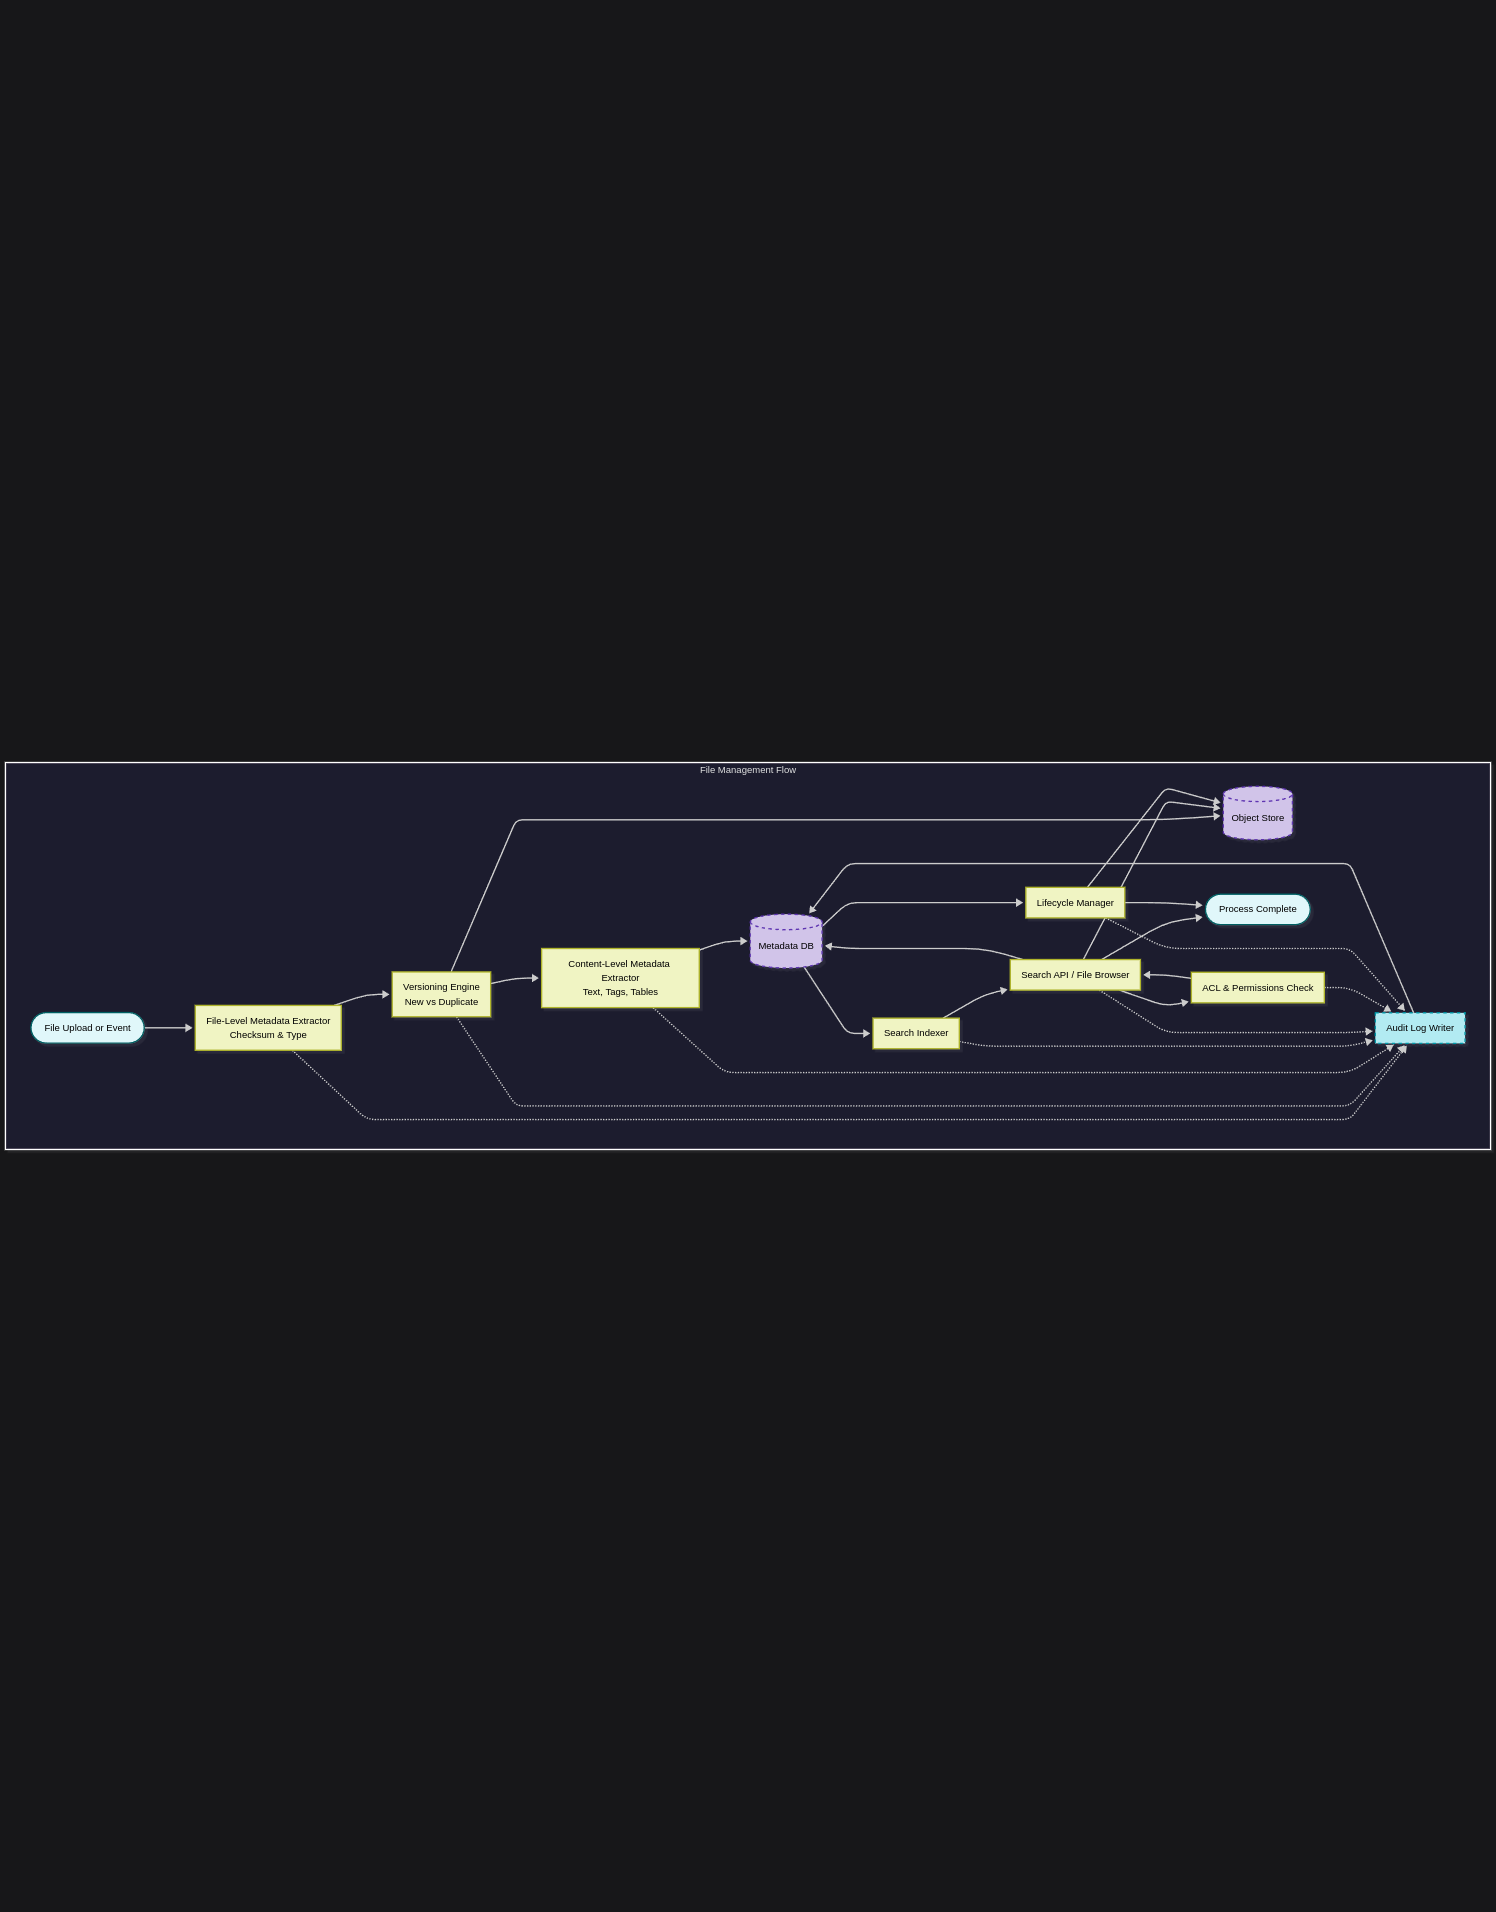
\includegraphics[width=0.5\textwidth]{store/flow.png} % Adjusted the scale of the image to 0.5
     
%     \end{figure}
% \end{frame}
% \begin{frame}{Components}
%     \begin{itemize}
%         \item \textbf{Object Store}: Store binary files such as documents, simulation files, AI outputs.
%         \item \textbf{Metadata DB}: Maintain file metadata, version history, project and task linkage.
%         \item \textbf{Vector Store}: Store and retrieve document embeddings for RAG-based agent prompts.
%         \item \textbf{Audit Log DB}: Log file events, agent actions, ERP task updates for analytics and compliance.
%         \item \textbf{Secrets Store}: Store per-project credentials, agent tokens, and access policies.
%         \item \textbf{Access API}: Unified internal API to upload, fetch, and version files and their metadata.
%     \end{itemize}
% \end{frame}

% % \begin{frame}
%     \frametitle{Technical Responsibilities}
%    \begin{table}[h!]
% \centering
% \renewcommand{\arraystretch}{1.2}
% \begin{tabular}{|p{3cm}|p{7cm}|}
% \hline
% \textbf{Component} & \textbf{Technical Responsibility} \\
% \hline
% Object Store & MinIO or S3-compatible blob storage, versioned uploads using unique keys \\
% \hline
% Metadata DB & Document and task metadata stored in MongoDB (document-style) or Postgres (relational) \\
% \hline
% Vector Store & Uses FAISS or Qdrant with HNSW or Flat index to store document embeddings \\
% \hline
% Audit Log DB & Uses TimescaleDB (Postgres extension) for time-series audit events and SLA logging \\
% \hline
% Secrets Store & Vault namespaces and paths store credentials and enforce RBAC policies per project \\
% \hline
% Access API & Exposes REST endpoints for file IO and metadata queries; supports access token validation \\
% \hline
% \end{tabular}
% \caption{Storage Layer - Technical Responsibilities}
% \end{table}

% \end{frame}